\documentclass[discrete.tex]{subfiles}

\begin{document}

\section{Некоторые определения из теории множеств. Прямое произведение, разбиение множеств. Мощность объединения}
\begin{definition}
  Пустое множество ($\varnothing$) - мно-во, которому $\nin$ ни один элемент
\end{definition}

\begin{definition}
  Число элементов мн-ва A - мощность $|A|$
\end{definition}

\begin{definition}
  Множество чисел от k до l обозначается $k:l$
\end{definition}

\begin{definition}
  Мн-во A - подмн-во мн-ва B ($A \subset B$), если каждый элемент из A принадлежит B
  \begin{figure}[H]
      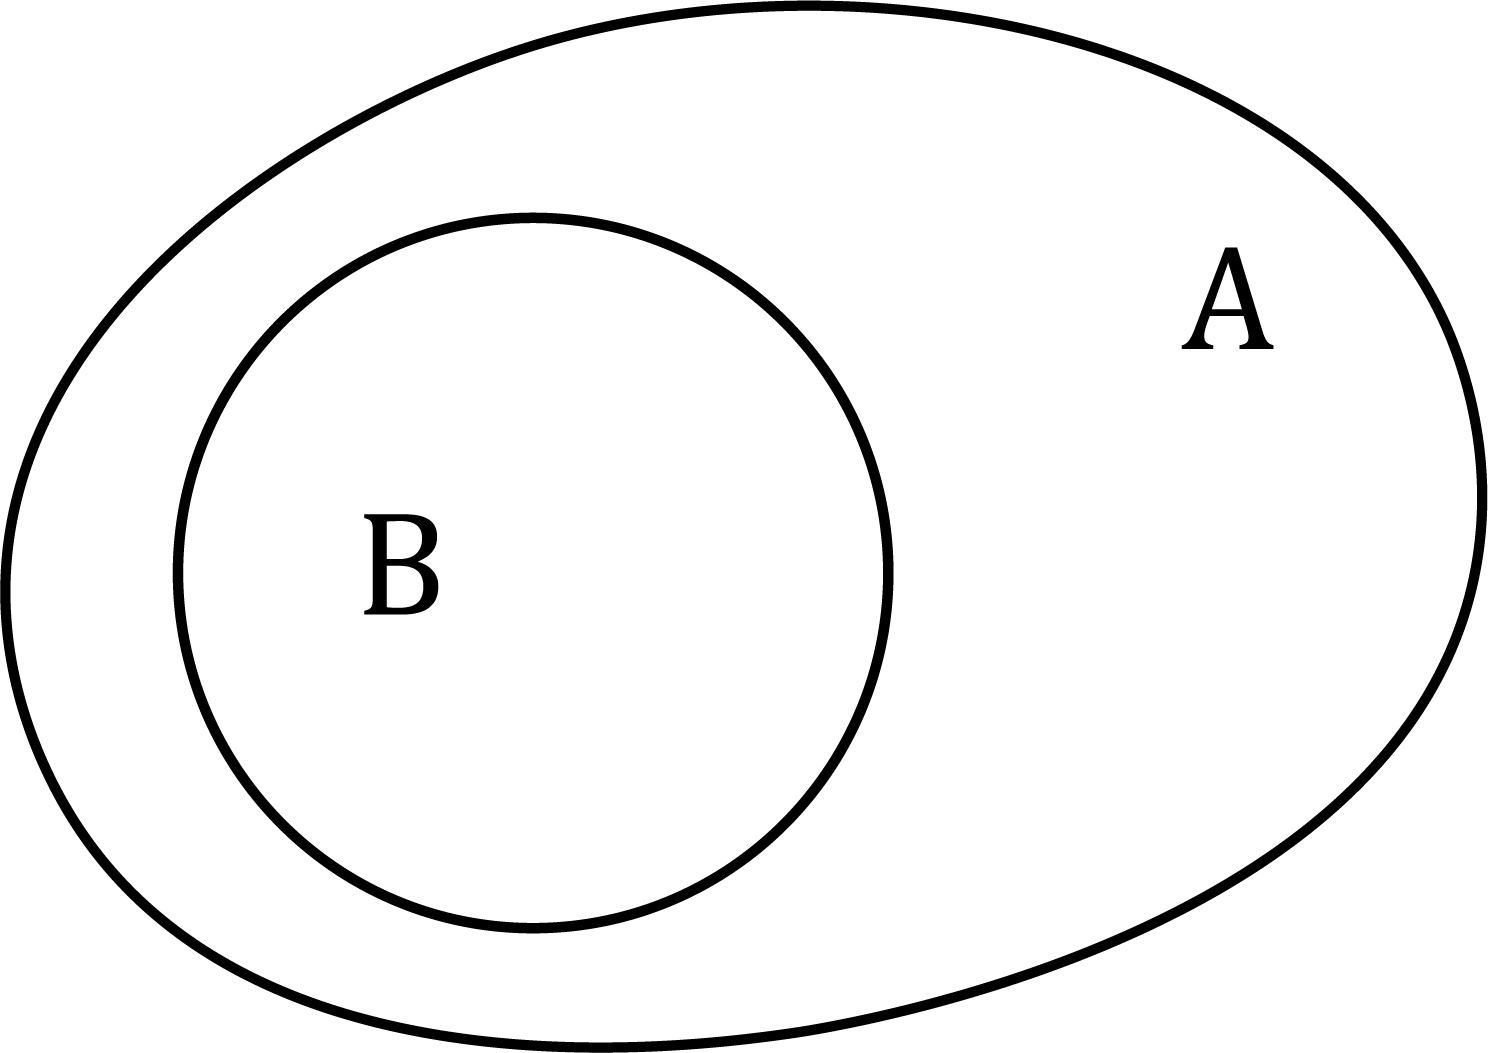
\includegraphics[width=4cm]{pics/1_1.png}
      \centering
  \end{figure}
\end{definition}

\begin{definition}
  C - объединение A и B ($A \cup B$), если оно состоит из всех элементов A и B ($C = \{x | x \in A \text{ и } x \in B\}$)
  \begin{figure}[H]
      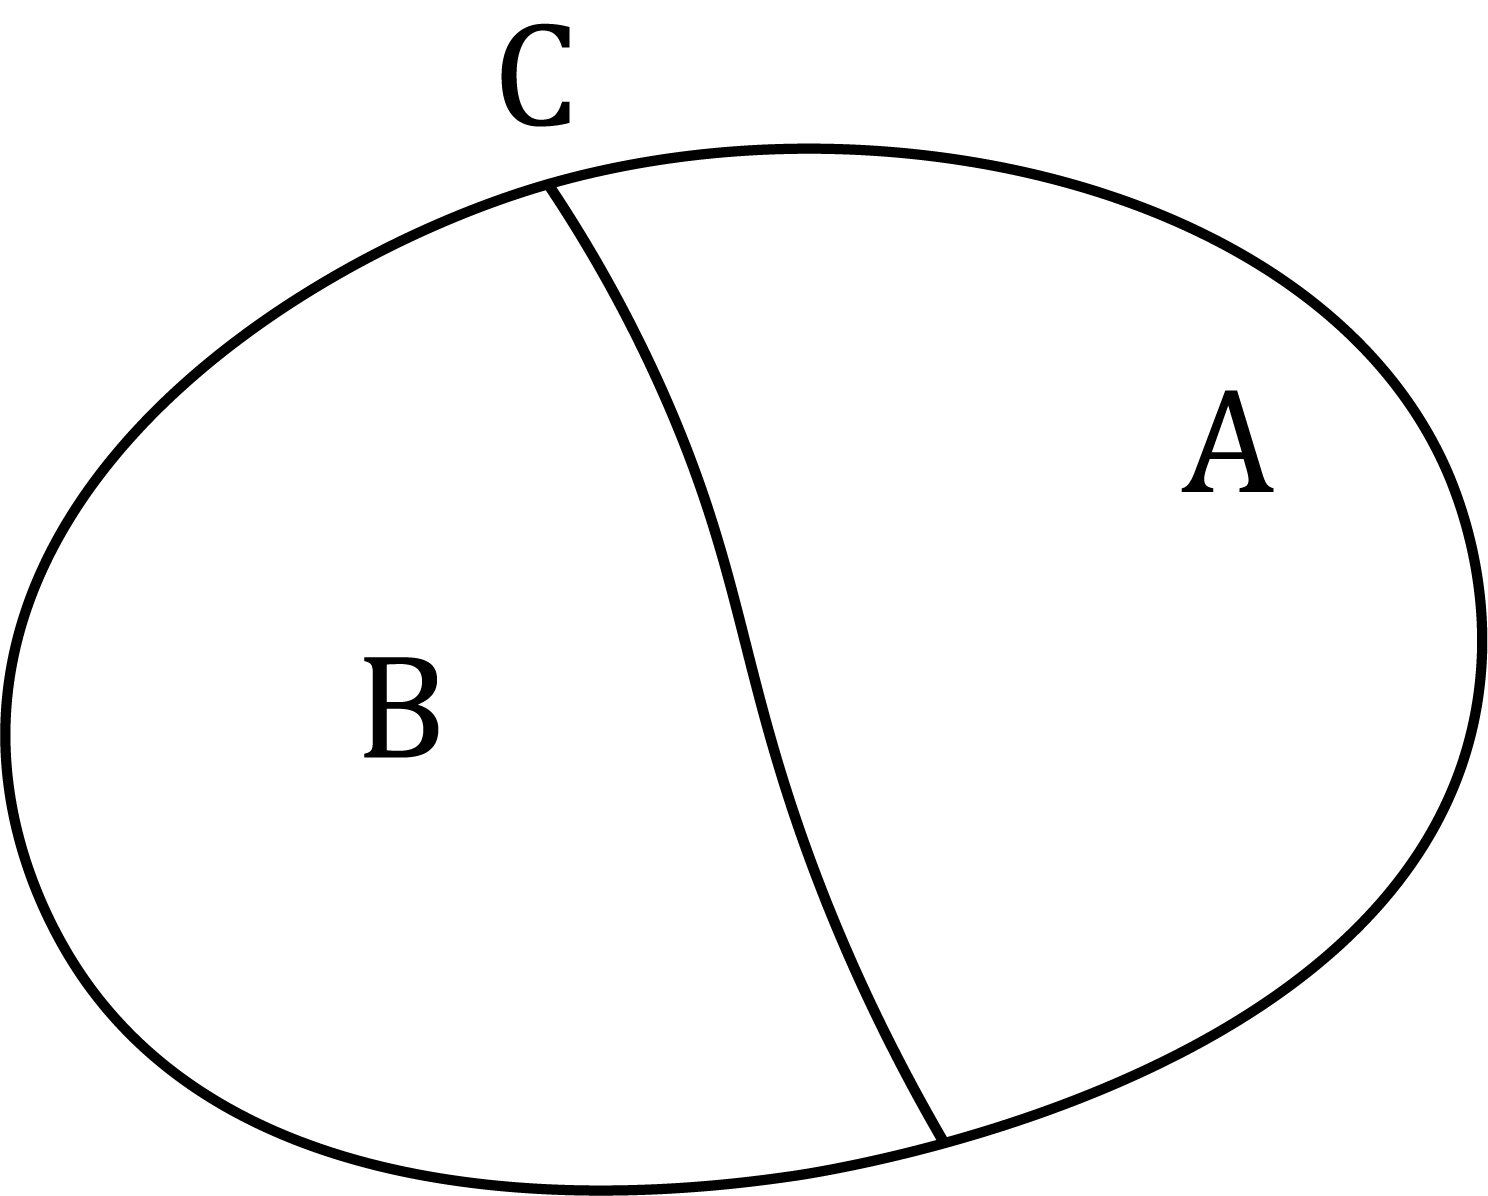
\includegraphics[width=4cm]{pics/1_2.png}
      \centering
  \end{figure}
\end{definition}

\begin{definition}
  $\us{i=1}{\os{n}{\cup}} A_i,\q \us{i=1}{\os{n}{\cap}} A_i$ - объединение и пересечение конечного числа мн-в
  \[(\us{i \in I}{\cup} A_i,\q \us{i \in I}{\cap} A_i) \text{ - аналогично}\]
  \begin{figure}[H]
      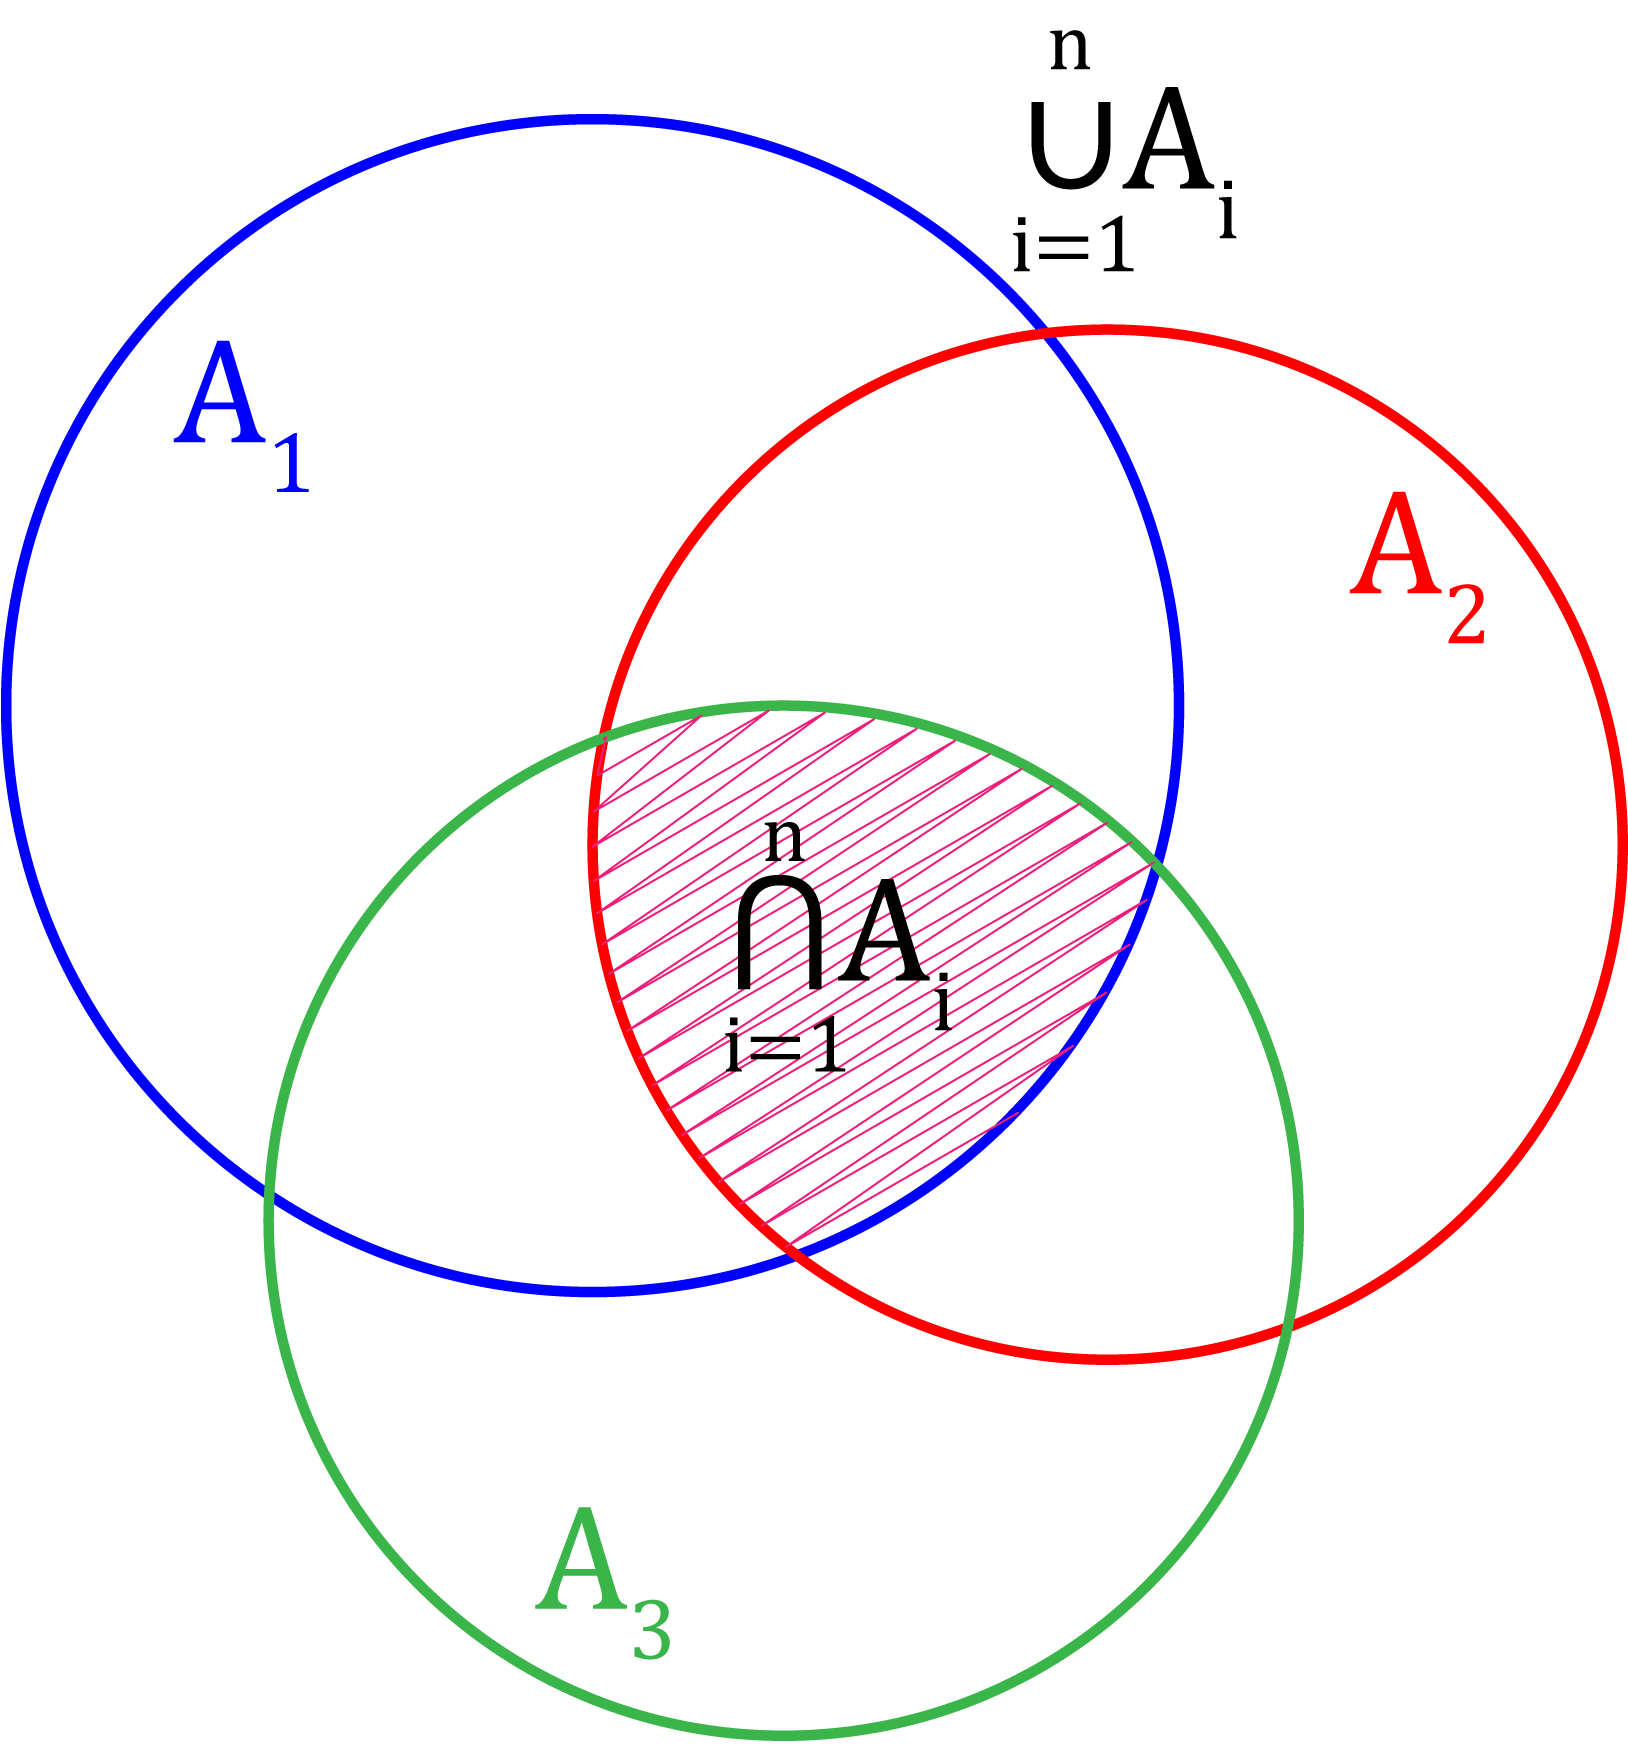
\includegraphics[width=5cm]{pics/1_3.png}
      \centering
  \end{figure}
\end{definition}

\begin{definition}
  Если пересечение мн-в пусто, то они называются дизъюнктивными
  \begin{figure}[H]
      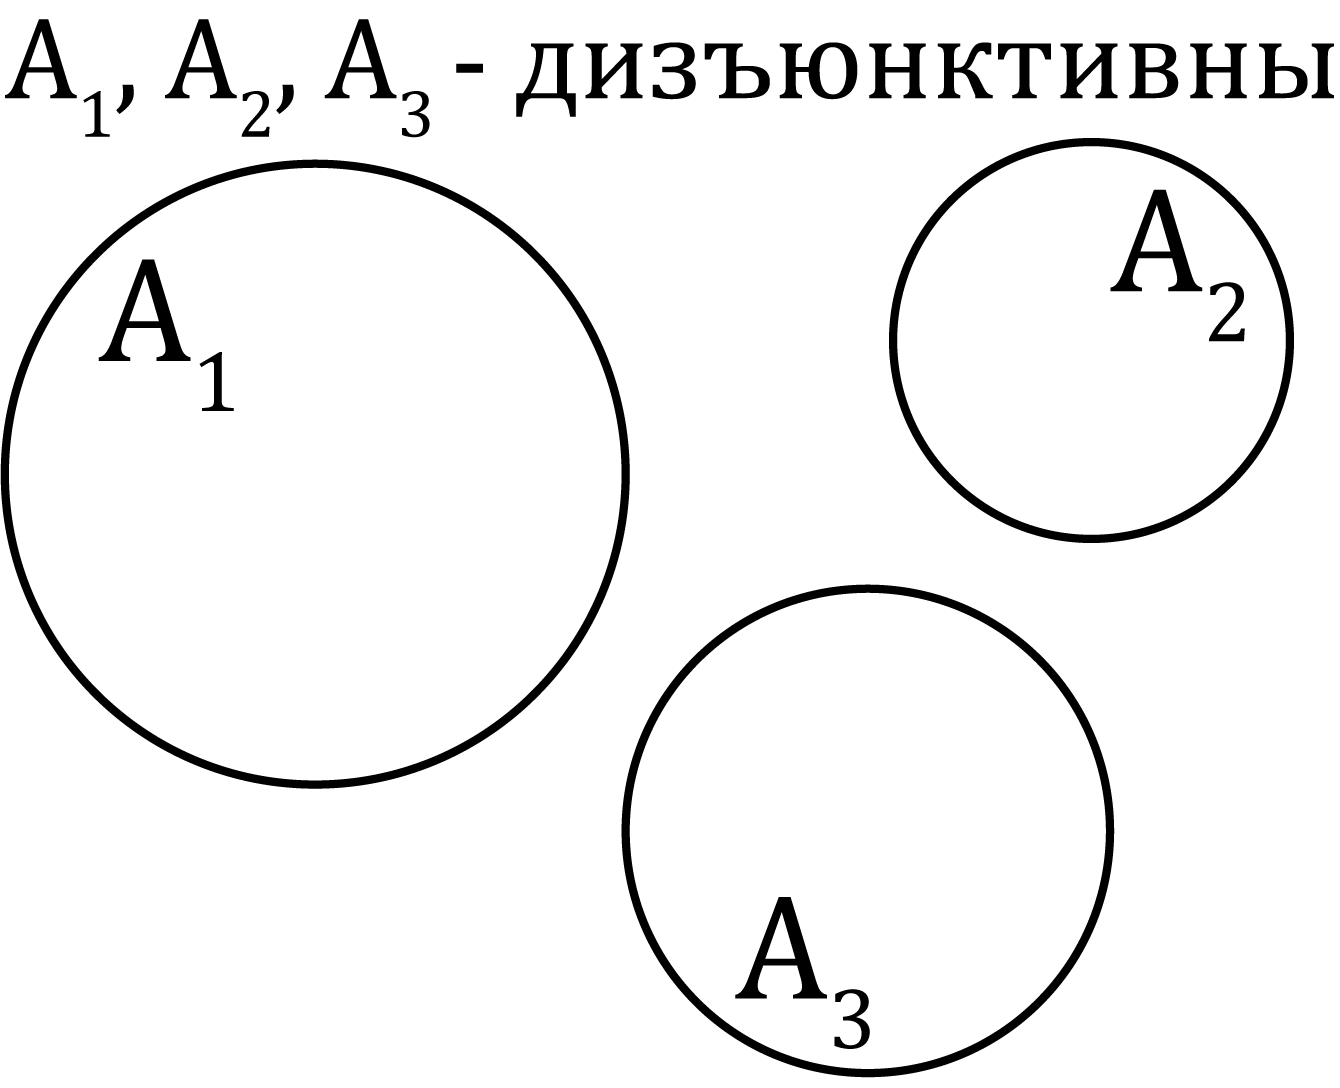
\includegraphics[width=5cm]{pics/1_4.png}
      \centering
  \end{figure}
\end{definition}

\begin{definition}
  Мн-во C называется разностью мн-в A и B ($C = A \setminus B$), если оно состоит из всех эл-в, принадлежащих А и не принадлежащих B
  \begin{figure}[H]
      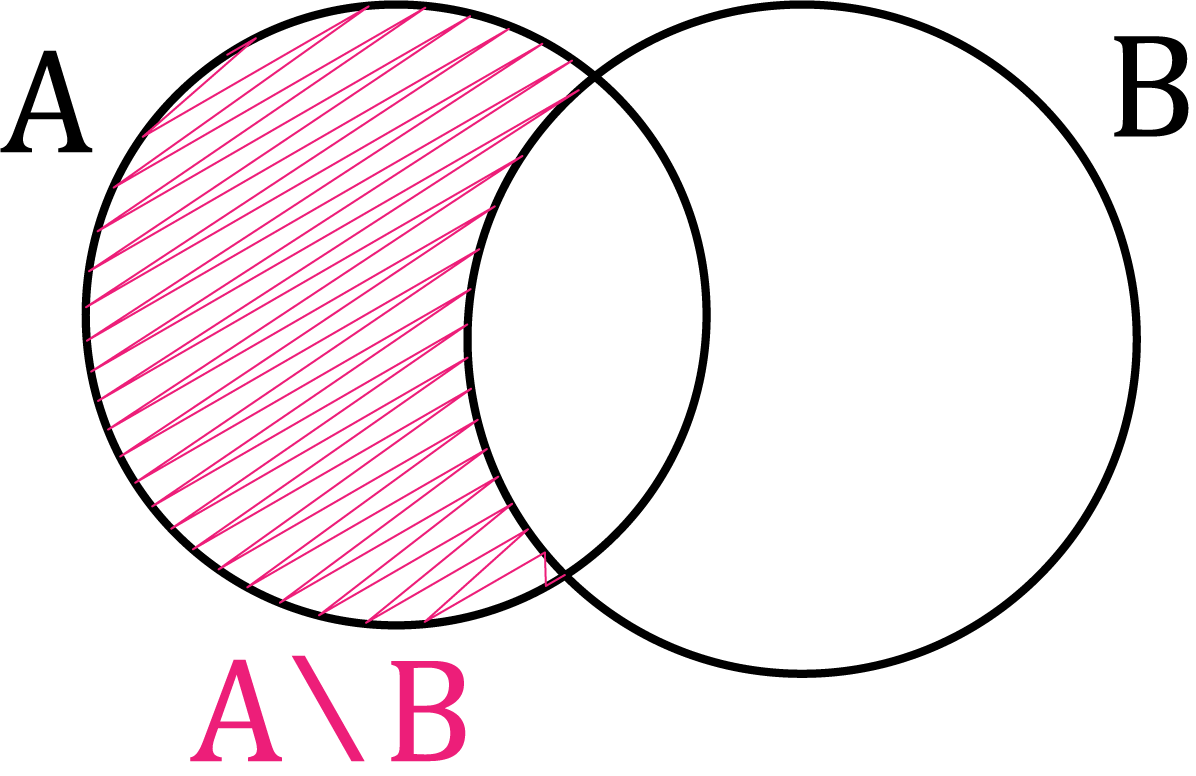
\includegraphics[width=5cm]{pics/1_5.png}
      \centering
  \end{figure}
\end{definition}

\begin{definition}
  $A \triangle B = A \setminus B \cup B \setminus A$ - симметрическая разность
  \begin{figure}[H]
      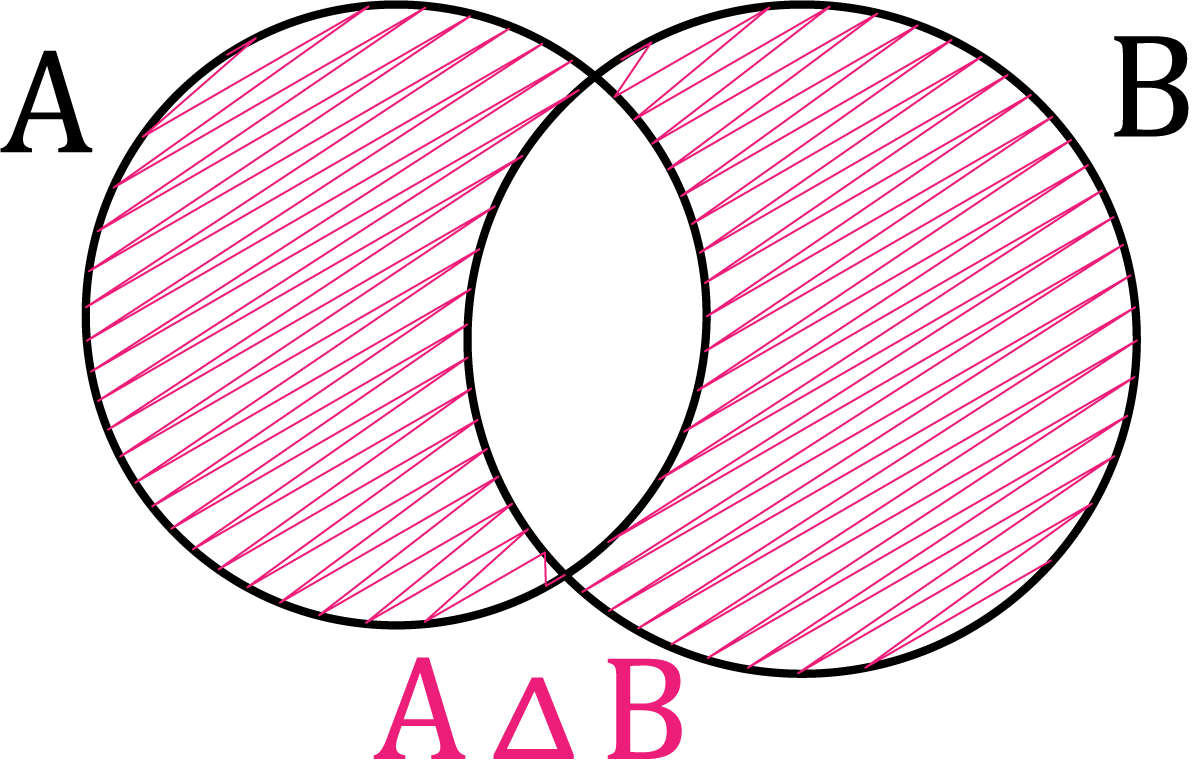
\includegraphics[width=5cm]{pics/1_6.png}
      \centering
  \end{figure}
\end{definition}

\begin{definition}
  Мн-во упорядоченных пар ($i,j$), где $i \in A$, $j \in B$ называется прямым произведением мн-в A и B
  \[A \times B = \{(i,j)\ |\ i \in A,\q j \in B\}\]
  \begin{figure}[H]
      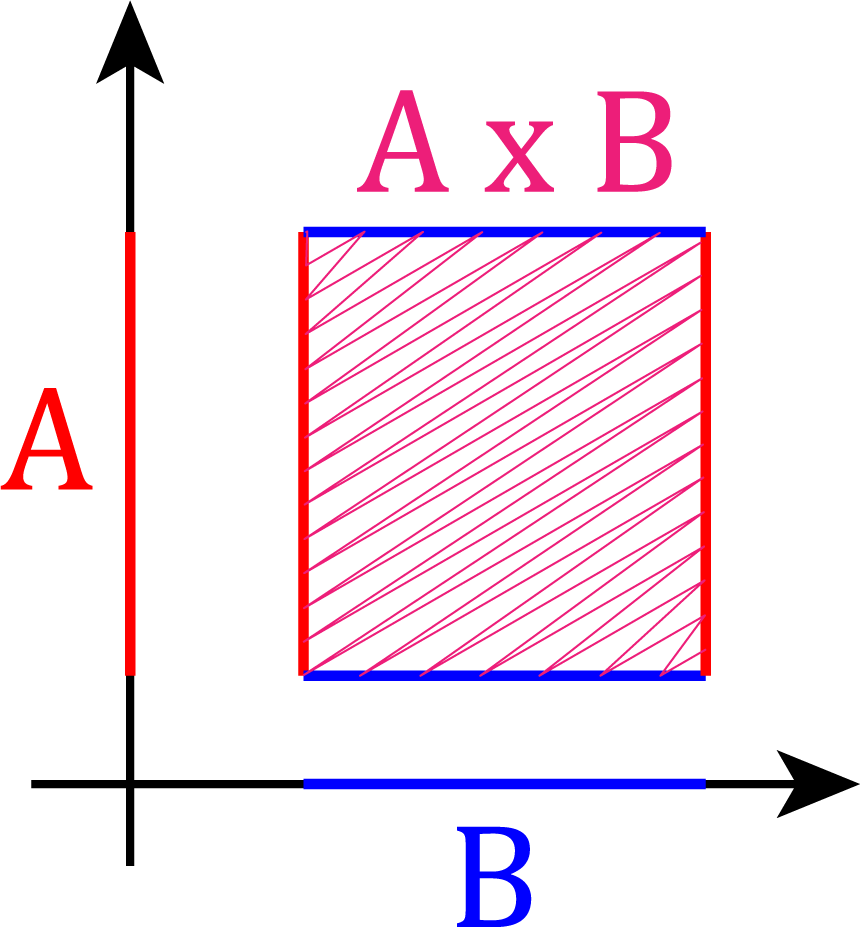
\includegraphics[width=3cm]{pics/1_7.png}
      \centering
  \end{figure}
\end{definition}

\begin{remark}
  Мощность прямого произведения $|A \times B| = |A| \cdot |B|$. Аналогично произведение $\forall$ конечного числа множеств
\end{remark}

\begin{definition}
  Пусть $A_1,...,A_k$ - ненулевые и попарно дизъюнктивные, $M = A_1 \cup ... \cup A_k$, тогда мн-во $\{A_1,...,A_k\}$ называется разбиением M\\
  (если они попарно не дизъюнктивные, тогда это покрытие)
  \begin{figure}[H]
      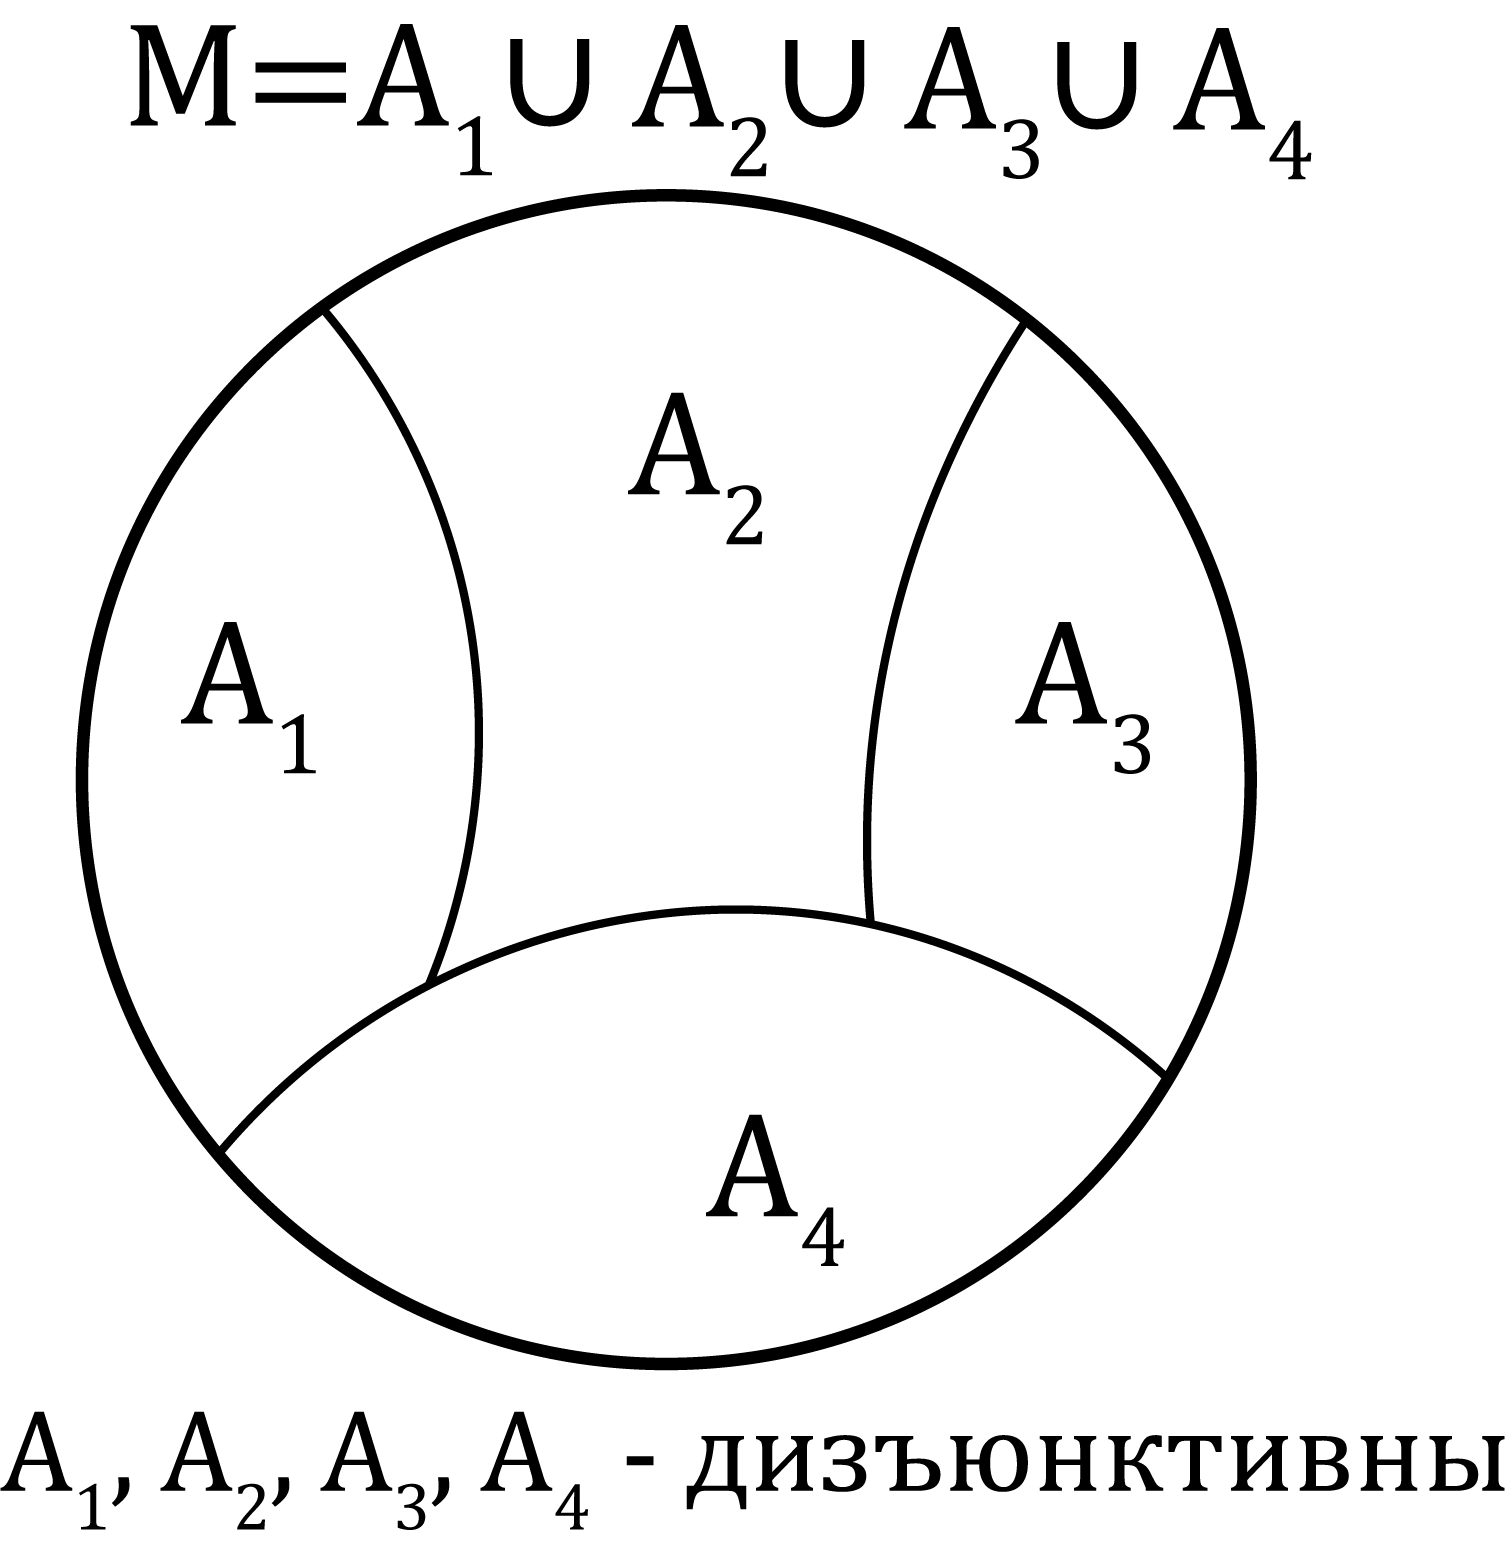
\includegraphics[width=5cm]{pics/1_8.png}
      \centering
  \end{figure}
\end{definition}

\begin{definition}
  Разбиение A мн-ва M называется измельчением B, если $\forall A_i \in A$ содержится в некотором $B_i \in B$
  \begin{figure}[H]
      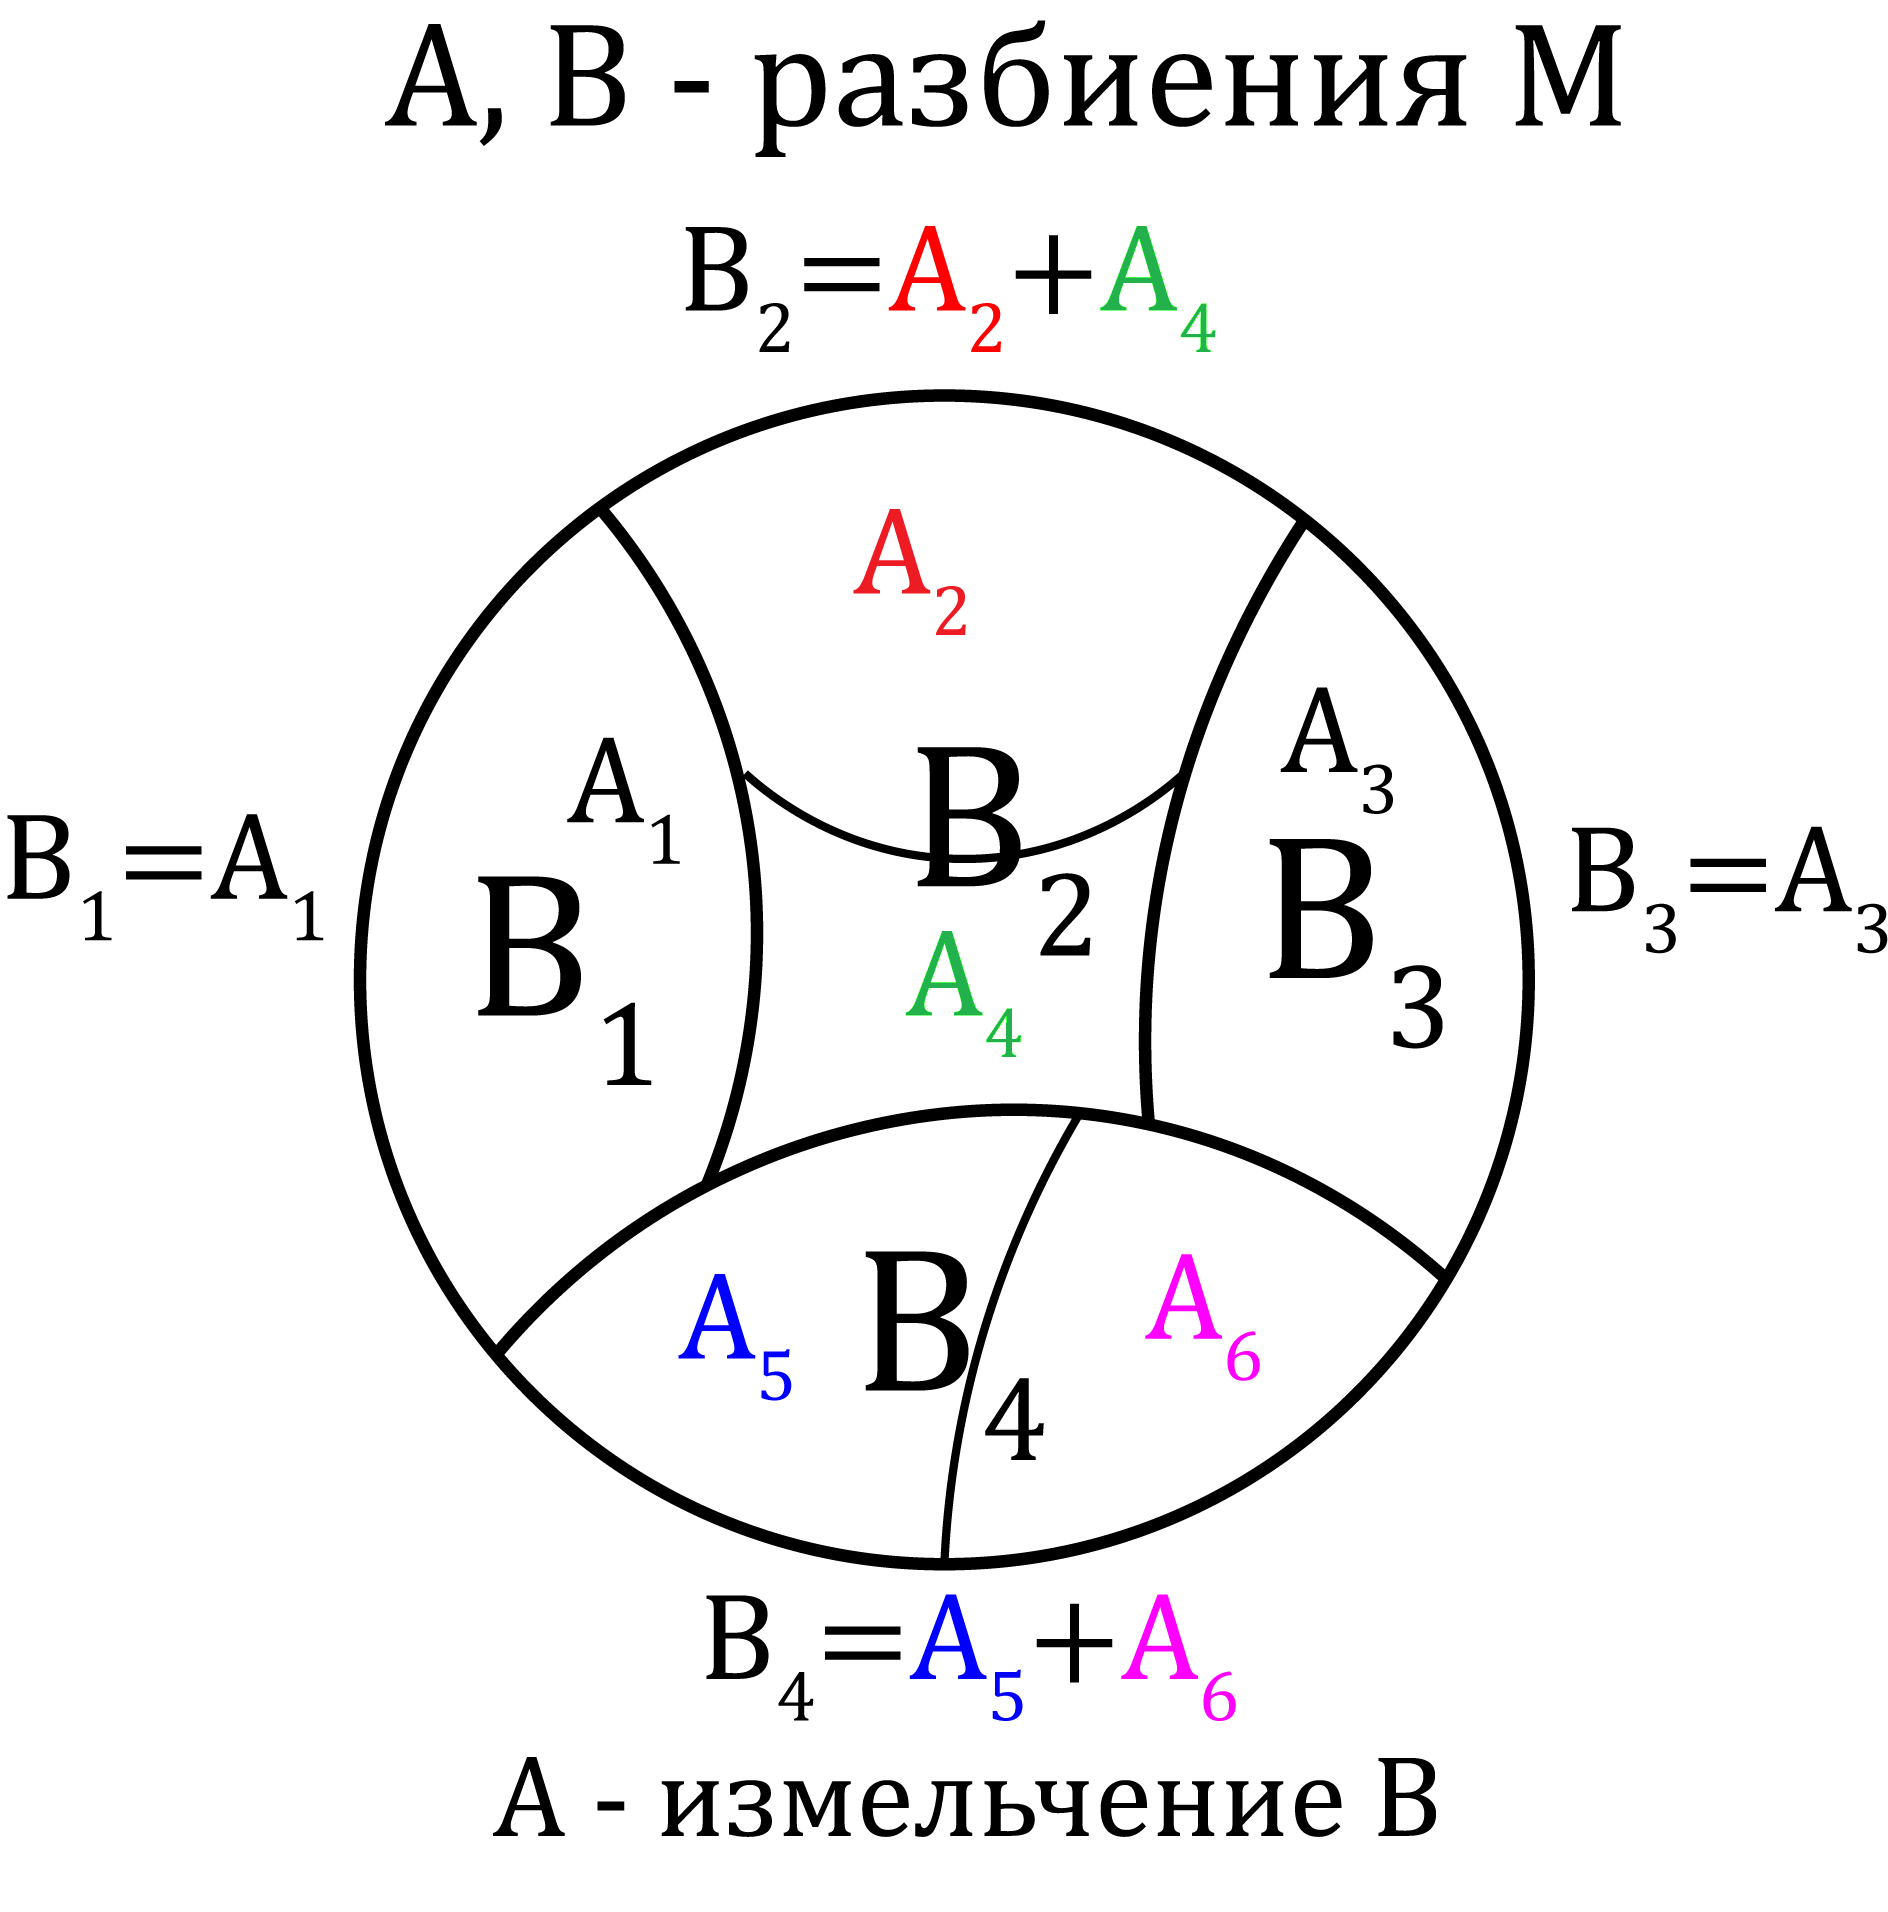
\includegraphics[width=5cm]{pics/1_9.png}
      \centering
  \end{figure}
\end{definition}


\begin{definition}
  Пусть A, B - размельчения мн-ва M, разбиение C называется произведением A и B, если оно является из измельчением, причем самым крупным $C = A \cdot B$
  \begin{figure}[H]
      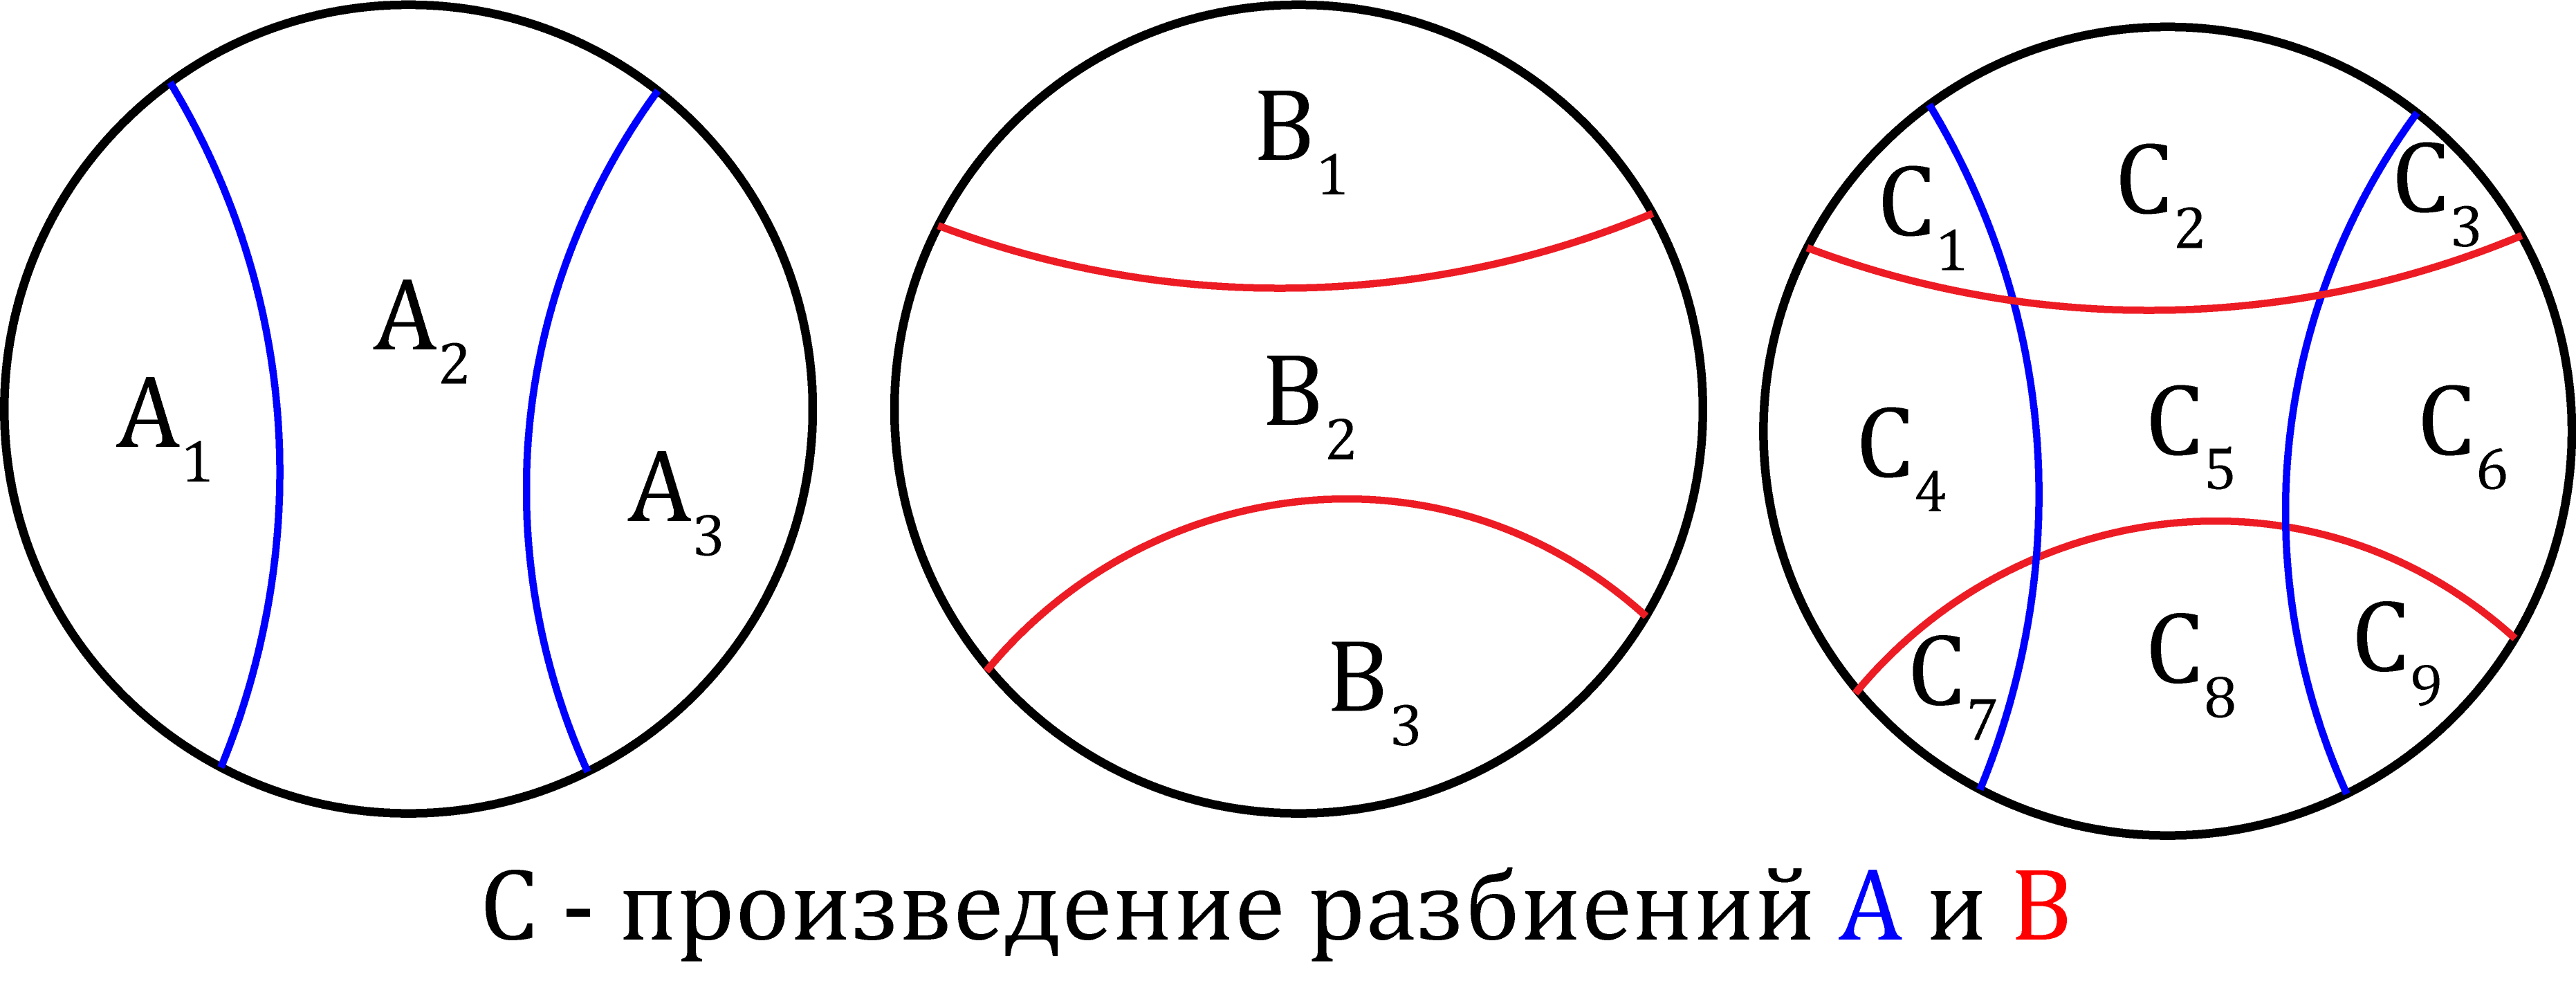
\includegraphics[width=10cm]{pics/1_10.png}
      \centering
  \end{figure}
\end{definition}

\begin{theorem}
  Произведение двух разбиений существует
\end{theorem}

\begin{proof}
  Предъявим разбиение, которое будет пересечением $A = \{A_1,...,A_k\}$ и $B = \{B_1,...,B_l\}$, точнее $D_{ij} = A_i \cap B_j,\q i \leqslant k,\q j \leqslant l$
  \[\Ra\mathcal{P} = \cup D_{ij} \text{ (т.е. без пустых строк)}\] Покажем, что тогда оно самое крупное

  Пусть $\e F = \{F_1,...,F_t\}$ - измельчение A и B, тогда:
  \[\forall F_k\q \e A_{i_k},\ B_{i_k}: F_k \subset A_{i_k},\ B_{i_k} \Ra F_k \subset (A_{i_k} \cup B_{i_k}) = D_{i_k j_k} \Ra \text{ мельче F}\]
\end{proof}

\end{document}
